%TODO: Add support for correlation with complex numbers

\section{Correlation function}

According to \citet{golomb_ref}, the correlation function measures how similar
two phenomena are. If properly normalized, the function ranges from
+1(identical) to -1(opposite); 0 meaning completly unrelated phenomena.
If we represent those phenomena as vectors, the correlation can be concived
as the normalized dot product between those 2 vectors.
In the discrete case where both sequences have the same length (the one we are
going to focus on), the normalized version is defined as follows:

\begin{definition}[Normalized correlation]\label{def:1}

Given $\alpha$ and $\beta$ two vectors of the same length n and $\alpha_{i}$
and $\beta_{i}$ the components of the vectors:

\begin{equation}\label{eq:1}
C(\alpha , \beta)=\frac{(\alpha \cdot  \beta)}{|\alpha||\beta|}=\frac{\sum_{i=1}^{n} \alpha_{i}\beta_{i}}{(\sum_{i=1}^{n} \alpha_{i}^{2})^{\frac{1}{2}}(\sum_{i=1}^{n} \beta_{i}^{2})^\frac{1}{2}}
\end{equation}
\end{definition}

Notice that in this vector
representation:
\begin{itemize}
  \item Orthogonal vectors have a correlation value of 0
  \item Vectors with the same direction and orientation have a correlation
  value of 1
  \item Vectors with the same direction but opposite orientation have a
  correlation value of -1
\end{itemize}

Even though the normalized version is the best way to represent the degree
of similarity between 2 phenomena and a good way to grasp the concept of
what we are defining, for the rest of the document we are going to use the
unnormalized version if not specified. This version of the correlation function
have several advantages for our research as it is simpler and carries the same
amount of information, saving us some computation resources and complexity on
our theoretical analysis. Keep in mind that it's always posible to move from
applied to the normalized one if we need it. The unnormalized correlation is
defined as:

\begin{definition}[Unnormalized correlation]\label{def:2}
  Given $\alpha$ and $\beta$ two vectors of the same length n and $\alpha_{i}$
  and $\beta_{i}$ the components of the vectors:
  \begin{equation}\label{eq:2}
    C(\alpha , \beta) = (\alpha \cdot  \beta) = \sum_{i=1}^n(\alpha \odot \beta)_{i}= \sum_{i=1}^{n} \alpha_{i}\beta_{i}
  \end{equation}

  Where "$\odot$" represents the pointwise product of vectors.

\end{definition}

Adapting this function from vectors to finite digital signals is straight
forward, as they can be defined in terms of a vector that lives in a vector
space of dimension equal to the length of the signal.


\begin{figure}[ht!] % [h!] fuerza que el elemento se sitúe
                    % en la posición señalada, en vez de al
                    % comienzo de una página.
\begin{center}
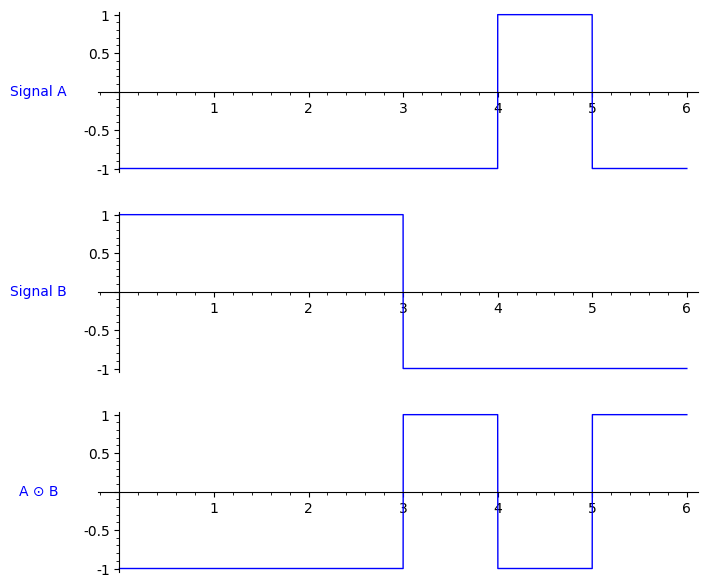
\includegraphics[width=0.7\linewidth]{Chapters/Introduction/signals_correlation}
\end{center}
\caption{Representation of 2 signals an their pointwise product with an unnormalized correlation between them of -2(-1 -1 -1 +1 -1 +1)}
\label{introduction_signals_hadamard}
\end{figure}

If we take a look at Figure \ref{introduction_signals_hadamard}, we can see
a simple computation that can easily be implemented in a chip. Notice that,
in contrast of what would be needed for the normalized version, we only use
integer arithmetics, multiplication and addition rather than squaring along the
signal proccesing and then calculating the square root.











\section{Autocorrelation function}

Going on with the lecture of \citet{golomb_ref}, the autocorrelation function
is a measure of how the correlation behaves if, for a given sequence, a
circular shift is applied and correlated with the original sequence for every
possible shift. It is defined for periodic sequences as follows:

\begin{definition}[Autocorrelation]\label{def:3}

Given the function C defined in Equation \ref{eq:2} and n the length of the
sequence S

\begin{equation}\label{eq:3}
  shift(S, \tau)_i = S_{(i+\tau) \bmod n}
\end{equation}
\begin{equation}\label{eq:4}
  A(S)_{\tau} = C(S, shift(S, \tau)) = \sum_{i=1}^{n}S_{i}S_{(i+\tau) \bmod n}
\end{equation}

\end{definition}

\begin{figure}[ht!] % [h!] fuerza que el elemento se sitúe
                    % en la posición señalada, en vez de al
                    % comienzo de una página.
\begin{center}
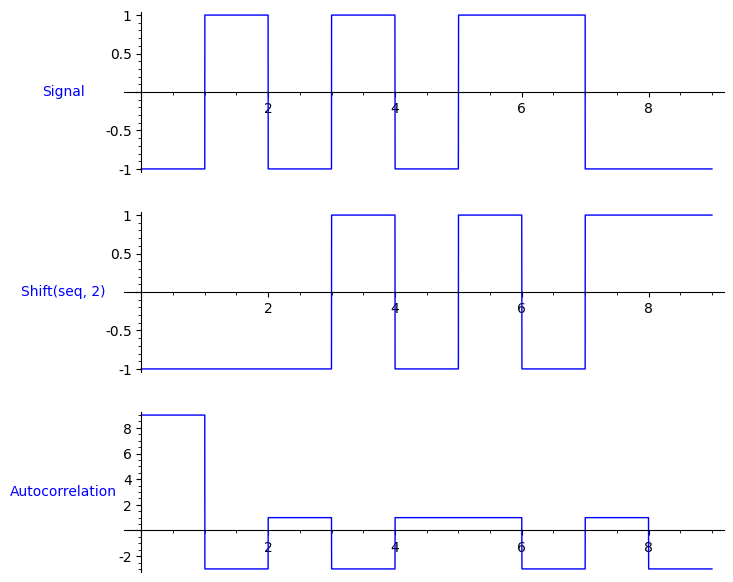
\includegraphics[width=0.7\linewidth]{Chapters/Introduction/signals_autocorrelation}
\end{center}
\caption{A signal with a shifted version of itself and it's autocorrelation function}
\label{introduction_signals_autocorrelation}
\end{figure}

An example of this function is shown in Figure
\ref{introduction_signals_autocorrelation} in which we can find examples of
some important properties of the autocorrelation function:

\begin{theorem}\label{theorem:1.2.1}
  Given a sequence S, the autocorrelation value for $\tau = 0$ is:
    \begin{equation}
      A(S)_{0}=C(S, S)=\sum_{i=1}^{n}S_{i}^2
    \end{equation}
\end{theorem}

\begin{corollary}
  Given the unnormalized autocorrelation of a sequence, we can
  normalize it by dividing it as follows:
  \begin{equation}
    A'(S)_{\tau} = \frac{A(S)_{\tau}}{A(S)_{0}}
  \end{equation}
\end{corollary}

\begin{proof}
  Using Equations \ref{eq:1} and \ref{eq:4}, we can normalize \ref{eq:4} as
  follows:

    $$A'(S)_{\tau} = C'(S, shift(S, \tau)) = \frac{C(S, shift(S, \tau))}{(\sum_{i=1}^{n} S_{i}^{2})^{\frac{1}{2}}(\sum_{i=1}^{n} S_{i+\tau}^{2})^\frac{1}{2}} = \frac{A(S)_{\tau}}{\sum_{i=1}^{n} S_{i}^{2}} = \frac{A(S)_{\tau}}{A(S)_{0}}$$

  Keep in mind that, even though $S_{i}^2$ and $S_{i+\tau}^2$ aren't the same element, the elements of the shifted version are the same as the original sequence so the total sum is the same.
\end{proof}

\begin{corollary}\label{autocorrelation:coro:1}
  Given the autocorrelation of a sequence, $A_{0}(S)$ will always be the maximum value of the autocorrelation.
\end{corollary}

\begin{property}
 Components of the autocorrelation vector belong to the same group as the
  original sequence.
\end{property}

Even though this seems a naive property, this will prove
useful when we introduce the algorithm based in the Fourier Transform to
compute the autocorrelation function.









\section{Crosscorrelation function}

The crosscorrelation function measures how a sequence correlates with all
the posible shifts of another sequence. This function is useful in signal
proccesing to analyze if two signals can be mistaken one for another by a
receiver.


\begin{definition}[Crosscorrelation]\label{def:4}
  Given C the correlation function defined in Equation \ref{eq:2}, shift as the function defined in Equation \ref{eq:3} and n the length of both sequences:
  \begin{equation}\label{eq:7}
    CC(S1, S2)_{\tau} = C(S1, shift(S2, \tau)) = \sum_{i=1}^{n}S1_{i}S2_{(i+\tau) \bmod n}
  \end{equation}
\end{definition}

\begin{figure}[ht!] % [h!] fuerza que el elemento se sitúe
                    % en la posición señalada, en vez de al
                    % comienzo de una página.
\begin{center}
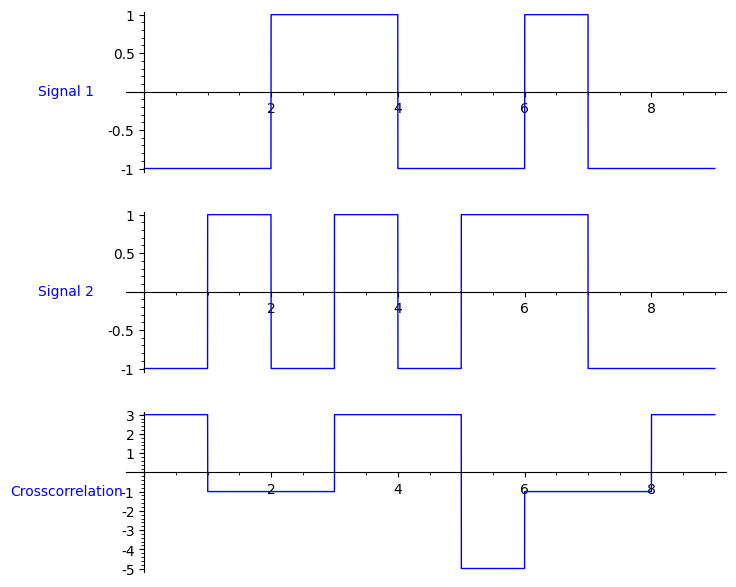
\includegraphics[width=0.7\linewidth]{Chapters/Introduction/signals_crosscorrelation}
\end{center}
\caption{Two signals and it's crosscorrelation}
\label{introduction_signals_crosscorrelation}
\end{figure}

\begin{lemma}\label{lem:1}
  Given a sequence S, CC the crosscorrelation function defined in Equation
  \ref{eq:7} and A the autocorrelation function defined in Equation \ref{eq:4}:
  \begin{equation}\label{eq:8}
    CC(S, S) = A(S)
  \end{equation}
\end{lemma}












\section{Pseudorandom noise(PRN)}

Noise have a different meaning depending on the field of study in which is
used. In our case we are going to work with random vectors of white noise,
which is defined as vectors in which all the components are statistically
independent between them.\cite{white_noise}\\

Even though noise in general is usually seen as an unwanted wave that
limits the amount of information that can be transmited through a
channel\cite{shannon_noise}, it has some practical uses:


\begin{outline}
  \1 PRN-based radars\cite{prn_radar_example1}\cite{prn_radar_example2}
  \1 As the spreading code in direct-sequence spread spectrum(DSSS) \cite{DSSS_1}\cite{DSSS}
    \2 CDMA in wireless communication\cite{DSSS}
    \2 GPS\cite{GPS}
\end{outline}

This practical applications exploit an important noise property:

\begin{property}
  The autocorrelation of a vector of white noise equals 0 for every component
  where $\tau \neq 0$ \cite{everett}
\end{property}

Taking a radar as an example, using this theorem can compute the distance
just by sending a white noise signal to a target and start correlating the
received signal with the original one. As the autocorrelation of
white noise only has a spike when the shift is 0, that spike represents in
which time instant the signal has returned. With that time instant, we can
get the round-trip time and then the actual distance if we know the
propagation speed of the wave.\\

In the case of GPS, the restrictions imposed to the noise sequence are
stronger. First of all, as we will be transmiting several signals in the same
frecuency, we need a set of codes with good crosscorrelation properties
between them. In other words, the crosscorrelation function between two given
codes must trend to 0 in every component, except when $\tau = 0$ and
both codes are the same.\\

As noise is an statistical construct, noise measured from natural phenomena
can generate sequences with poor correlation properties. As both technologies
depend on this properties to work, we must find a way of creating sequences
with properties similar to those of noise in an deterministic and efficient
fashion.\\

This kind of sequences are called Pseudorandom Noise(PRN). In practical
applications, PRN sequences aren't perfect noise because generating it is
difficult and unnecesary. In reality, we don't need an actual 0 in every
position of the autocorrelation. If we let the sequence take values in a
threshold so that the system won't mistake intermidiate values with the
autocorrelation spike, it will behave as expected.

\begin{figure}[ht!] % [h!] fuerza que el elemento se sitúe
                    % en la posición señalada, en vez de al
                    % comienzo de una página.
\begin{center}
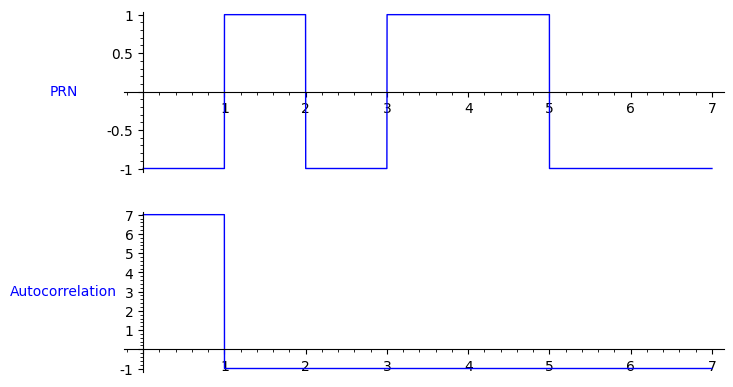
\includegraphics[width=0.7\linewidth]{Chapters/Introduction/signals_prn}
\end{center}
\caption{A pseudorandom noise sequence an it's autocorrelation function.
Notice that this PRN code isn't perfect noise.}
\label{introduction_signals_autocorrelation}
\end{figure}

% TODO Define family of sequences

% TODO Define flat autocorrelation
